\chapter{Marco Conceptual}
\label{chap:marco_conceptual}

En este capítulo se describen los conceptos necesarios para que el lector se pueda familiarizar con los conceptos usados en el resto del informe, describiendo lo que se entiende por los conceptos usados en términos de redes sociales y conceptos asociados al desarrollo de la solución.\\

En caso de así preferirlo, el lector puede saltar las secciones que estime convenientes dentro de este capítulo, en caso de dominar los conceptos y usar este capítulo como referencia en caso de necesitarlo.

\section{Conceptos de Redes Sociales} % (fold)
\label{sec:conceptos_de_redes_sociales}


A continuación se expondrán los conceptos fundamentales que se usarán en la memoria en relación a redes sociales. Estos conceptos fueron tomados de la tesis de doctorado del alumno del DCC, Mauro San Martín\cite{tesismauro}, que representan lo necesario para el entendimiento de este trabajo. Su reuso e inclusión en el informe se hace sólo para que el lector no necesite revisar la memoria de Mauro para poder ver estos conceptos.

Para construir la definición formal de redes sociales, es necesario definir algunos conceptos claves previamente, siguiendo las definiciones clásicas de este dominio\cite{sna}.

\subsection{Actor} % (fold)
\label{sub:actor}
Un actor es una entidad social, la cual está bajo estudio junto con sus interacciones sociales. En estricto rigor, los actores pueden ser definidos como individuos, corporaciones o unidades sociales colectivas. Ejemplos de actores son gente en un grupo, departamentos en una empresa o agencias de servicio público en una cuidad. El uso del término actor no significa que estas entidades necesariamente tienen la habilidad de actuar. Más allá, la mayoría de las aplicaciones en redes sociales se enfocan en colecciones de actores que son de un mismo tipo (por ejemplo, gente en un grupo de trabajo). A veces, sin embargo, la investigación necesita mirar a actores de diversos niveles o tipos conceptuales, o desde diversos conjuntos. Los datos pueden incluir atributos no relacionales asociados a los diferentes actores.
% subsection actor (end)

\subsection{Vínculos Relacionales} % (fold)
\label{sub:vinculos_relacionales}
Los actores están conectados hacia otros por vínculos sociales. El rango y tipo de estos puede ser muy amplio. La característica principal de un vínculo es que establece una conexión entre un par de actores. Algunos de los ejemplos más comunes de vínculos empleados en el análisis de redes sociales son:

  \begin{itemize}
    \item La evaluación de una persona por otra, ej: amistad declarada, gusto o respeto.
    \item Transferencia de recursos materiales, ej: transacciones de negocios, prestar o pedir prestado.
    \item Asociación o afiliación, ej: atender conjuntamente a un evento social, o pertenecer al mismo club social.
  \end{itemize}
% subsection vinculos_relacionales (end)

\subsection{Relaciones} % (fold)
\label{sub:relaciones}
El conjunto de vínculos entre un tipo específico de miembros de un grupo se llama una relación. Por ejemplo, el conjunto de las amistades entre pares de niños en un salón de clases, o el conjunto de uniones diplomáticas entre pares de naciones en el mundo, son vínculos que definen relaciones. Para cualquier grupo de actores, podemos encontrar diversas relaciones; por ejemplo, además de las relaciones diplomáticas entre países, podemos encontrar la existencia de comercio en un determinado año. Las relaciones (o vínculos específicas) pueden tener atributos que las describen. Por ejemplo en el caso del comercio, su cantidad de transacciones total puede haber sido almacenado.
% subsection relaciones (end)

Con lo expuesto anteriormente, finalmente podemos definir una red social.

\subsection{Red Social} % (fold)
\label{sub:red_social}
Una red social consiste en uno o muchos conjuntos finitos de actores, junto con las relaciones definidas entre ellos. La presencia de información relacional es una característica crítica de las redes sociales. Una red social es un caso particular de red, de esta manera su estructura puede ser formalizada como un grafo.

En adición al uso de conceptos relacionales (Wasserman y Faust\cite{sna}) se deben tener en cuenta las siguientes consideraciones:

  \begin{itemize}
    \item Actores y sus acciones son vistos como interdependientes, más que independientes, unidades autónomas.
    \item Vínculos relacionales (conexiones) entre actores son canales de transferencia o "flujo" de recursos (material o no material).
    \item Modelos de red enfocados en individuos muestran el ambiente estructural de la red, además de proveer la capacidad de definir limitaciones en nivel individual.
    \item Los modelos de red conceptualizan estructura (social, económica, política, entre otras) como patrones generales de relaciones entre actores.
  \end{itemize}
% subsection red_social (end)


% ### 2.1 Conceptos de Redes Sociales
% 
% * explicación de que se van a reusar (copiar-pegar casi) los conceptos de redes sociales de la tesis de mauro
% 
% #### 2.1.1. Definiciones
% 
% * red social
% * nodo {NO}
% * actor
% * atributo {NO}
% * relación
% * familia {NO}
% * rol {NO}

% {NO} es pq estos conceptos son más específicos al modelo de mauro, pues se entienden mejor con el modelo

\section{Conceptos de Desarrollo} % (fold)
\label{sec:conceptos_de_desarrollo}

% TODO: ver que dijo claudio aquí en XXXXXXX
A continuación se explican los términos referentes al desarrollo de XXXXXXX del trabajo realizado en esta memoria.

\subsection{Desarrollo Web} % (fold)
\label{sub:desarrollo_web}

% * que es el desarrollo web
% * arquitectura de cliente servidor
% * que componentes típicos se encuentran en el desarrollo web
%   * servidor
%   * browser
%     * web
%     * movil
%   * servidor de bases de datos
%   * servidor de acceso a aplicaciones

El desarrollo web se denomina al desarrollo de software cuyo fin es la creación de aplicaciones que se ejecuten en computadores que puedan ser accesados vía la \emph{world-wide web}. Este estilo de desarrollo conlleva a que una aplicación que pueda estar ejecutándose en un servidor pueda entregar resultados a clientes provenientes de cualquier parte del mundo, usando una gran diversidad de dispositivos, plataformas de software, etc. Esas aplicaciones son frecuentemente accesadas por personas vía un navegador web.\\

Esta propiedad de multiplataforma de las aplicaciones desarrolladas para la web, junto con propiedades de accesibilidad desde diversos medios a las aplicaciones, ha hecho que el desarrollo web sea un enfoque de desarrollo ampliamente usado en la industria en los últimos 10 años.\\

En términos generales el desarrollo web posee una arquitectura clásica de cliente/servidor, en donde una aplicación corriendo en un servidor proporciona resultados y ejecuta instrucciones proveniente de clientes, que pueden ir desde un navegador web de p.c. o dispositivo móvil, o servir de API, \emph{Application Programming Interface}, para otras aplicaciones. A continuación se adjunta un diagrama que muestra los principales componentes cuando se habla de desarrollo web.\\

% TODO agregar figura de elementos en el desarrollo web

A modo de ejemplo de componentes en el desarrollo web de una aplicación que posee un servidor de ejecución de la aplicación, con un servidor de base de datos, que es accesada vía teléfono, tablet o computador por medio de un navegador web o de una interfaz API que use otra aplicación, por la cual se acceden sus datos en formato de documentos HTML (junto con sus estilos en CSS y manejo de eventos en JavaScript) o documentos en formato JSON, RDF, XML entre otros.\\

Dentro del desarrollo web, también se encuentran subcategorías que son expuestas a continuación.

\subsubsection{Desarrollo Front-End} % (fold)
\label{ssub:desarrollo_front_end}
% * es el desarrollo que compone todos los aspectos de un sistema con los cuales interactúa un cliente, como el cliente
% la arquitectura de cliente-servidor

Es el desarrollo orientado a todos los componentes con los cuales interactúa un usuario de la aplicación, enfocado en la interfaz y sus componentes gráficos, además de la experiencia usuario, la usabilidad de la aplicación, etc. Es el desarrollo del cliente que el usuario usa para acceder al core de la aplicación.\\

En términos de tecnologías, se asocia el desarrollo front-end al uso de tecnologías como: HTML, CSS, Javascript, entre otras.
% subsubsection desarrollo_front_end (end)

\subsubsection{Desarrollo Back-End} % (fold)
\label{ssub:desarrollo_back_end}

% * es desarrollo de software de la aplicación que guarda y procesa los datos del usuario

Es el desarrollo de la aplicación que almacena y posee la lógica común a todos los clientes de la aplicación, en donde el código de este tipo de desarrollo se ejecuta en el servidor. Además generalmente en el desarrollo back-end se incluye todo lo relacionado a persistencia de datos generados a través del uso de la aplicación.

% subsubsection desarrollo_back_end (end) 
% subsection desarrollo_web (end)

\subsection{Modelo MVC} % (fold)
\label{sub:modelo_mvc}
El modelo MVC (Modelo, Vista, Controlador)\cite{mvc}, consiste en un modelo para separar la lógica de una aplicación agrupándola en clases u otras unidades modulares, de acuerdo con la responsabilidad que estos módulos cumplan dentro de un sistema. A modo de ejemplo, a fin de ilustrar este concepto, se puede dar un caso de una aplicación que registre compras en un sistema de tienda online, un ejemplo de los módulos asociados a compras en MVC puede ser el siguiente:

\begin{figure}[!h]
  \centering
  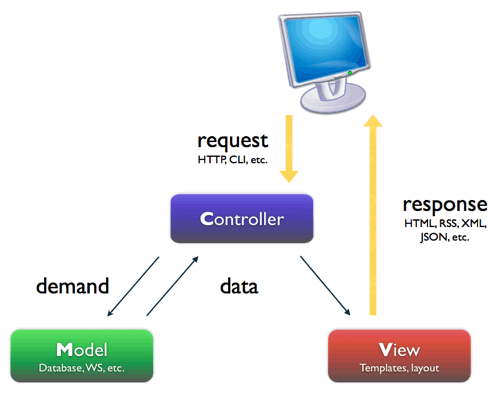
\includegraphics[scale=.5]{images/mvc.png}
  \caption{Modelo MVC}
  \label{modelomvc}
\end{figure}

\begin{itemize}
  \item \textbf{Modelo}: el modelo corresponde a una clase \texttt{Compra} que contiene toda la lógica de negocio asociada a las compras, que además se asocia directamente a cómo se almacena una compra en la base de datos.
  \item \textbf{Vista}: un ejemplo de vista para una compra, puede ser una interfaz \texttt{HTML} en la cual el cliente efectúe operaciones sobre la compra, por ejemplo agregar productos, cabe destacar que la vista no ejecuta las acciones, sólo se encarga de recibirlas y enviarlas al último componente del modelo MVC, el controlador.
  \item \textbf{Controlador}: de acuerdo a lo recién expresado, el controlador es el encargado de coordinar uno o más modelos para ejecutar las acciones capturadas en la vista. En el caso de la compra, el controlador es quien efectivamente procesaría el pago de la misma.
\end{itemize}
% subsection modelo_mvc (end)

\subsection{Frameworks de Desarrollo} % (fold)
\label{sub:frameworks_de_desarollo}
Un framework de desarrollo define un marco en el cual desarrollar una aplicación. Provee una gran cantidad de funcionalidad común lista de manera de no desarrollar un proyecto desde cero, pero además de funcionalidad, provee de una estructura lógica con la cual se escribe el código, que está influida por muchas otras personas que han usado el framework en aplicaciones reales.

\subsubsection{Frameworks Server Side} % (fold)
\label{ssub:frameworks_server_side}
Dentro de los frameworks de desarrollo web existe una categoría llamada \emph{Sever Side}, la cual consiste en que el código de la aplicación corre desde un servidor en internet, lo que permite que si la computación es común para muchos clientes, los resultados de esa computación pueden ser usados múltiples veces.\\

Ejemplos actuales de esta categoría de frameworks son: \texttt{Ruby on Rails}\cite{rails}, \texttt{Sinatra}\cite{sinatra} que utilizan el lenguaje \texttt{Ruby}; \texttt{Django}\cite{django}, \texttt{Pylons}\cite{pylons} para \texttt{Python}; \texttt{Spring}\cite{spring} para \texttt{Java} y \texttt{CakePHP}\cite{cake} para PHP entre otros.
% subsubsection frameworks_server_side (end)

\subsubsection{Frameworks Client Side} % (fold)
\label{ssub:frameworks_client_side}
En el último tiempo, surgió una nueva categoría de frameworks de desarrollo web llamada \emph{Client Side}, en la cual el código de la aplicación se ejecuta en el computador del usuario de la aplicación, ahorrando recursos necesarios en un servidor, además de ahorrar el tiempo de latencia entre el cómputo de una respuesta y su transmisión al equipo del usuario.\\

Comúnmente estos frameworks son escritos para ser usados con el lenguaje \texttt{Javascript}, pues posee la propiedad que todos los navegadores web implementan un motor de \texttt{Javascript} y por lo tanto el usuario no necesita instalar nada más. Ejemplos de frameworks client side son: \texttt{AngularJS}\cite{angular}, \texttt{EmberJS}\cite{ember}, \texttt{Meteor}\cite{meteor} y alternativamente \texttt{BackboneJS}\cite{backbone} que es una librería más que un framework.
% subsubsection frameworks_client_side (end)

% subsection frameworks_de_desarollo (end)

% #### 2.2.5. HTML5
% 
% * a que se llama HTML5
% * que entrega a diferencia de las versiones anteriores
% 
% ##### 2.2.5.1 SVG, Gráficos Vectoriales en la Web
% 
% * que son y de que sirven estos gráficos (redimensión, formato común xml, etc)
\subsection{HTML5} % (fold)
\label{sub:html5}

\emph{Html5}\cite{html5} es el nuevo estándar para \emph{HTML} (Hyper-Text Markup Language), definido por la WC3\cite{w3c} y Web Hypertext Application Technology Group (WHATWG), es un trabajo en progreso, sin embargo desde hace tiempo los principales navegadores soportan muchas de los nuevos elementos de HTML y sus APIs.\\

Algunas de los nuevas características más interesantes en HTML5 son: el tag \texttt{<canvas>} para dibujo en 2D, los tags \texttt{<video>} y \texttt{<audio>} para reproducción multimedia, soporte para almacenamiento local en el browser, algunos elementos específicos para el contenido como \texttt{<article>}, \texttt{<footer>}, \texttt{<header>}, \texttt{<nav>} y \texttt{<section>}; nuevos controles para formularios como para fecha, hora, email, url y búsqueda. Además de esto, soporte para SVG dentro de los sitios, característica especialmente importante para esta memoria.

\subsubsection{SVG, gráficos vectoriales en la web} % (fold)
\label{ssub:svg_graficos_vectoriales_en_la_web}

SVG, en inglés se refiere a gráficos vectoriales escalables, los cuales pueden ser usados directamente en documentos HTML5, de manera de crear gráficos complejos en un formato de tipo XML. La diferencia de este tipo de gráficos con respecto a imágenes por ejemplo, es que los gráficos SVG no pierden calidad si son redimensionados o se ven sus detalles por medio de una funcionalidad de lupa. Estos elementos son altamente animables y corresponde a una recomendación por parte de la W3C\cite{w3c}.

% subsubsection svg_gráficos_vectoriales_en_la_web (end)

% subsection html5 (end)

% section conceptos_de_desarrollo (end)

\section{Herramientas Elegidas} % (fold)
\label{sec:herramientas_elegidas}

A continuación se presentan las herramientas elegidas para el desarrollo de la aplicación y los fundamentos de estas elecciones:

\subsection{Ruby on Rails} % (fold)
\label{sub:ruby_on_rails}
Para el desarrollo del backend de la aplicación se eligió el framework de desarrollo web Ruby on Rails\cite{rails}, comúnmente conocido simplemente como Rails, en el cual se desarrolla sobre el lenguaje Ruby. Es un framework maduro con 10 años de existencia, el cual es una de las plataformas más populares para este tipo de desarrollo actualmente en Silicon Valley.\\

Dentro de las características destacables de rails se pueden destacar: sus principios de privilegiar las convenciones sobre las configuraciones, es decir, el framework entrega mucha funcionalidad hecha mientras se cumplan sus convenciones, las cuales de ser necesario se pueden sobre escribir; aplicaciones que pueden ser ejecutadas en diversos ambientes independientemente configurados como producción, testing o desarrollo.\\

Además de aspectos técnicos, dentro de las motivaciones al elegir rails, se encuentra la presencia de una gran comunidad de desarrolladores que crean muchas librerías, o en terminología ruby, 'gemas' las cuales hacen el desarrollo mucho más rápido reusando estas librerías que resuelven múltiples problemas frecuentes. Junto con lo anterior el alumno memorista posee vasta experiencia laboral en esta tecnología.
% subsection ruby_on_rails (end)

\subsection{EmberJS} % (fold)
\label{sub:emberjs}

EmberJS es un framework de desarrollo web javascript en el lado del cliente, fue creado por Yehuda Katz y Tom Dale cuando ellos hacían la segunda versión del framework web Sproutcore.\\

EmberJS se destaca debido a que se pueden escribir aplicaciones completas que son ejecutadas en el lado del cliente, con clases especializadas como \emph{modelos}, \emph{vistas}, \emph{controladores}, \emph{templates} en una versión un poco distinta del modelo MVC. Una característica principal de emberjs es la actualización automática de templates cuando la información el sistema cambia; la presencia de observadores y la capacidad de adaptar emberjs a diversos modelos de persistencia como vía API JSON o el almacenamiento local integrado en los navegadores web de última generación.\\

Para el desarrollo de la aplicación de esta memoria, debido a que se trata de una aplicación que permite editar grafos interactivamente y es vía web, es necesaria mucha integración entre el javascript de las vistas y los datos de los nodos de las redes sociales, razón por la cual fue un mejor enfoque desarrollar la aplicación con emberJS, que resultó en pruebas iniciales mucho mejor que la otra alternativa evaluada, BackboneJS\cite{backbone}.\\

Uno de los aspectos útiles de EmberJS es que uno de sus creadores, Yehuda Katz, es integrante de los equipos principales de desarrollo de Ruby on Rails y la librería de javascript jQuery. De esta forma, EmberJS está pensado para tener una muy buena integración con Rails y jQuery, potenciando su atractivo como herramienta de desarrollo en el lado del cliente.

% subsection emberjs (end)

\subsection{D3.js} % (fold)
\label{sub:d3_js}

Dentro de las herramientas principales se incluye D3.js\cite{d3}, que es una librería javascript para el despliegue y manipulación de datos como información visual vía SVG en la web. Además de lo anterior D3.js es una de las opciones más utilizadas en lo que a gráficos SVG en la web se refiere.\\

El funcionamiento básico de D3 es el siguiente: se parte por asociar un arreglo de elementos que contienen los datos con los que trabajamos y son asociados con elementos SVG, como círculos por ejemplo y para el caso del arreglo de datos, D3 tiene 3 estados: el de entrada, es decir, cuando un elemento nuevo es agregado al arreglo, D3 se encarga de crear un nuevo elemento SVG para asociarlo a este nuevo dato; el estado de actualización  es el cual que a todos los datos disponibles actualiza su posición u otras propiedades y finalmente el estado de salida es cuando un elemento del arreglo es eliminado y por consiguiente D3.js se encarga de remover su elemento SVG respectivo.

% subsection d3_js (end)
